\documentclass[a4paper]{article}
\usepackage{geometry}
 \geometry{
 a4paper,
 total={210mm,297mm},
 left=1.25in,
 right=1.25in,
 top=1.25in,
 bottom=1.25in,
 }
\usepackage{graphicx}
\usepackage{todonotes}
\usepackage{tgpagella}
\usepackage[T1]{fontenc}
\usepackage{amsmath}
\usepackage{amssymb}
\usepackage{float}
\usepackage{subcaption}
\usepackage[caption = false]{subfig}
\newcommand{\argmax}{\operatorname{argmax}}

\begin{document}
\title{Traffic Sign Classification}
\author{Sasank - 110070051, Tharun - 10070048, Rajeev - 110070055}
\date{\today}
\maketitle

\section{Introduction}
We classify traffic sign images from German Traffic Sign Recognition Database using different methods. We used following algorithms
\begin{itemize}
\item Linear Discriminant Analysis (LDA)
\item Fisher's Linear Discriminant/Fisherfaces
\item Random Forests
\end{itemize}
We applied these on images and histogram of oriented gradients descriptors.

\section{Dataset}
We used German Traffic Sign Recognition Database for training and testing our classifiers. The dataset features 43 different signs under various sizes, lighting conditions, occlusions and is similar to real-life data.
Training set includes about 39000 images while test set has around 12000 images. Images are \emph{not} guaranteed to be fixed dimensions and sign is \emph{not} necessarily centred in each image. Each image contains a 10\% border around the actual traffic sign. However, annotations are provided for bounding box if we wish to remove this border. More details on the dataset can be found in \cite{dataset}



\begin{figure}
\begin{subfigure}{.5\textwidth}
  \centering
  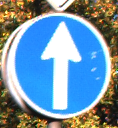
\includegraphics[scale = 2]{a.png}
  \caption{}
  \label{fig:sfig1}
\end{subfigure}%
\begin{subfigure}{.5\textwidth}
  \centering
  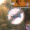
\includegraphics[scale = 2]{b.png}
  \caption{}
  \label{fig:sfig2}
\end{subfigure}
\begin{subfigure}{.5\textwidth}
  \centering
  
\includegraphics[scale = 2]{c.png}
  \caption{}
  \label{fig:sfig2}
\end{subfigure}
\begin{subfigure}{.5\textwidth}
  \centering
  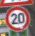
\includegraphics[scale = 2]{d.png}
  \caption{}
  \label{fig:sfig2}
\end{subfigure}
\begin{subfigure}{.5\textwidth}
  \centering
  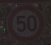
\includegraphics[scale = 2]{e.png}
  \caption{}
  \label{fig:sfig2}
\end{subfigure}
\begin{subfigure}{.5\textwidth}
  \centering
  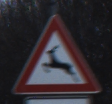
\includegraphics[scale = 2]{f.png}
  \caption{}
  \label{fig:sfig2}
\end{subfigure}

\caption{Samples of images from dataset, scaled to double the size}
\label{fig:fig}
\end{figure}


%\missingfigure{ one image each from each sign}

\section{Classification using Images}
In this section, we describe methodology used for classification using images directly. Bounding box of traffic sign provided in annotations is used to crop each image and it is converted to grey scale. Then images are rescaled to $40\times 40$ and are reshaped to $1 \times 1600$ row vector. Such row vector for each image are stored in a matrix $X$ and corresponding labels/classes in $y$.

\subsection{Linear Discriminant Analysis \cite{textbook}} \label{sec:LDA}
We use linear discriminant analysis on $X$ and $y$ to classify images. i.e, It is assumed that a sample vector from each class comes from a multivariate Gaussian distribution with different means $\mu_k$ but with same covariance matrix $\Sigma$ and with a prior probability of $\pi_k$. Since, we do not know $\mu_k,\pi_k$ and $\Sigma$, they have to estimated from the training data $(X,y)$
\begin{itemize}
\item $\hat{\pi}_k = N_k/N$ where $N_k$ is the number of class-$k$ observations
\item $\hat{\mu}_k = \sum_{y_i = k}{x_i/N_k}$
\item $\hat{\Sigma} = \sum_{k = 1}^{K}\sum_{y_i = k} (x_i-\hat{\mu}_k)^T(x_i-\hat{\mu}_k)/(N-K) $
\end{itemize}
where $x_i$ is $i$th row of $X$ and $N$ and  $K$ are total number of observations in training data and number of classes respectively. Calculation of $\Sigma_k$ can be vectorized as 
\[\hat{\Sigma} = \sum_{k = 1}^{K} (X_k-1*\hat{\mu}_k)^T(X_k-1*\hat{\mu}_k)/(N-K)\] 
where $1$ is matrix of ones of appropriate dimension and $X_k$ is matrix with rows from $X$ for which $y_i = k$ 

Once $\mu_k,\pi_k$ and $\Sigma$ are estimated, we can use Bayes classification. This can be shown to be equivalent to
\[
\hat{y}(x) = \argmax_k x\Sigma^{-1}\mu_k^T - \mu_k\Sigma^{-1}\mu_k^T/2 + \log{\pi_k}
\]
This computation can also be vectorized and further optimizations are possible to make this computation faster. However, we stop with vectorization as it is fast enough for our applications. Note that decision boundaries from this scheme are linear.

\subsubsection{Results}
This gives the worst classification of all the algorithms we implemented. This is because we do not expect raw image data to be linearly separable.
\begin{center}
\begin{tabular}{ |c|c|c| } 
 \hline
 Correctly classified & Misclassified & Total test images \\ 
 \hline
 $8539$ & $4091$ & $12630$ \\ 
 \hline
 $63.61 \%$ & $36.39 \%$ & $100 \%$ \\ 
 \hline
\end{tabular}
\end{center}

\subsection{Fisher's Linear Discriminant/Fisherfaces \cite{fischerfaces}}
This method selects a linear transformation $W$ such that the ratio of the between-class scatter and the within-class scatter is maximized. Between-class scatter matrix is defined as 
\[
S_B = \sum_{k=1}^{K} N_k(\mu_k - \mu)^T(\mu_k - \mu)
\]
Within-class scatter matrix is defined as 
\[
S_W = \sum_{k=1}^{K} \sum_{y_i = k}(x_i - \mu_k )^T(x_i - \mu_k)
\]
Here $\mu$ is mean of all images in training set.

If $S_W$ is non sigular, the optimal projection is chosen as the
\[
W_{opt} = \argmax_W \frac{|W^TS_BW|}{|W^TS_WW|} = [\mathbf{w_1} \mathbf{w_2} \dots \mathbf{w_m}]
\]
where $\mathbf{w_i}$ are generalized eigenvectors of $S_B$ and $S_W$ corresponding to $m$ largest eigenvalues $\lambda_i$.

Usually $S_W$ is singular. This is because rank of $S_W$ is at most $N-K$ and $N$, number of training images, is usually much smaller than number of pixels $n$ in each image. If so, PCA is done to reduce dimensions of data to $N-K-1$ before applying FLD.

In our case, $N - K = 32609 - 43 = 32566$ is much larger than number of pixels in each image $40\times 40 = 1600$. So, $S_W$ is invertible and generalized eigenvectors can be used to find $W_{opt}$.


Once $W_{opt}$ is found, we project each image in the training set using $W_{opt}$ and save them in a database. For a given test image, we project it onto the vector space and class corresponding to nearest neighbour in the database is returned as prediction.

\subsubsection{Results}
There is a considerable improvement in performance compared to LDA.
\begin{center}
\begin{tabular}{ |c|c|c| } 
 \hline
 Correctly classified & Misclassified & Total test images \\ 
 \hline
 $10914$ & $1716$ & $12630$ \\ 
 \hline
 $86.41 \%$ & $13.59 \%$ & $100 \%$ \\ 
 \hline
\end{tabular}
\end{center}

\section{Histogram of Oriented Gradients (HOG) \cite{hog}}
These are feature set originally proposed in \cite{hog} to detect humans in an image. However these can also be used for classification/detection of other objects like cars or traffic signs.

The basic idea is that local object appearance and shape can often be characterized rather well by the distribution of local intensity gradients or edge directions, even without precise knowledge of the corresponding gradients or edge positions. 
This is implemented by dividing the image window into small spatial regions (`cells'), for each cell accumulating a local 1-D histogram of gradient directions or edge orientations over the pixels of the cell. It is also useful to contrast-normalize the local responses before using them. This can be done by accumulating a measure of local histogram `energy' over somewhat larger spatial regions (`blocks') and using the results to normalize all of the cells in the block

\begin{figure}[h]
\centering

\includegraphics[scale = 0.75]{hog1.png}
\caption{Visualization of histogram of oriented gradients}
\end{figure}
Three sets of precomputed HOG descriptors are provided with dataset. To compute these features, each image is scaled to $40 \times 40$ pixels and following sizes of cells and overlapping blocks are used.

\begin{center}
\begin{tabular}{ |c|c|c|c|c| } 
 \hline
 Name & cell size & block size &  binning resolution & length  \\ 
 \hline
 HOG 1 & $5\times 5$ & $2\times 2$ & $8$ (sign ignored)& 1568\\ 
 \hline
 HOG 2 & $5 \times 5$ & $2\times 2$ & $8$ & 1568 \\ 
 \hline


\end{tabular}
\end{center}

\section{Classification using HOG descriptors}
Precomputed HOG vectors are used for classification for both LDA and FLD. There's a substantial improvement in performance.
\subsection{LDA Results}
\begin{center}
\begin{tabular}{ |c|c|c|c| } 
 \hline
 Descriptor &Correctly classified & Misclassified & Total test images \\ 
 \hline
 HOG 1 &$11766$ ($93.16 \%$) & $864$ ($6.84 \%$) & $12630 ($100 \%$)$ \\
\hline
 HOG 2 &$11766$ ($95.68 \%$) & $545$ ($4.32 \%$) & $12630 ($100 \%$)$ \\
 \hline


\end{tabular}
\end{center}

\subsection{FLD Results}
\begin{center}
\begin{tabular}{ |c|c|c|c| } 
 \hline
 Descriptor &Correctly classified & Misclassified & Total test images \\ 
 \hline
 HOG 1 &$11766$ ($ 94.32 \%$) & $717$ ($5.68 \%$) & $12630 ($100 \%$)$ \\
\hline
 HOG 2 &$12197$ ($96.57 \%$) & $433$ ($3.43 \%$) & $12630 ($100 \%$)$ \\
 \hline

\end{tabular}
\end{center}

\begin{figure}
\begin{subfigure}{.5\textwidth}
  \centering
  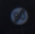
\includegraphics[scale = 2]{1.png}
  \caption{}
  \label{fig:sfig1}
\end{subfigure}%
\begin{subfigure}{.5\textwidth}
  \centering
  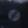
\includegraphics[scale = 2]{2.png}
  \caption{}
  \label{fig:sfig2}
\end{subfigure}
\begin{subfigure}{.5\textwidth}
  \centering
  
\includegraphics[scale = 2]{3.png}
  \caption{}
  \label{fig:sfig2}
\end{subfigure}
\begin{subfigure}{.5\textwidth}
  \centering
  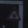
\includegraphics[scale = 2]{4.png}
  \caption{}
  \label{fig:sfig2}
\end{subfigure}
\begin{subfigure}{.5\textwidth}
  \centering
  
\includegraphics[scale = 2]{5.png}
  \caption{}
  \label{fig:sfig2}
\end{subfigure}
\caption{Some Misclassified Images when LDA is applied on HOG 1 descriptors}
\end{figure}

\section{Random Forests (RF)\cite{textbook}}
We apply technique of random forests on HOG descriptor data to classify signs. Random forests are ensemble of bagged randomized decision trees in which a random set of features are selected for best split. Each randomized decision trees above is trained with bootstrap sample of training data. i.e, sample of same size as training data is drawn from training data picking each sample uniformly randomly \emph{with replacement}.

\subsection{Results}
Our implementation of RF gives very bad results. This is because splits are premature at each node. We couldn't debug this. These are the results from sklearn package's RandomForestClassifier class. Number of trees in the ensemble trained are 50.
\begin{center}
\begin{tabular}{ |c|c|c|c| } 
 \hline
 Descriptor &Correctly classified & Misclassified & Total test images \\ 
 \hline
 HOG 1 &$11709$ ($  92.70 \%$) & $921$ ($7.30 \%$) & $12630 ($100 \%$)$ \\
 \hline
\end{tabular}
\end{center}

\section{Improvements possible}
Our random forests code was not able to find good splits. We could've debugged this had we had more time.


\begin{thebibliography}{4}
\bibitem{dataset} 
Man vs. computer: Benchmarking machine learning algorithms for traffic sign recognition, \emph{J. Stallkamp, M. Schlipsing, J. Salmen, C. Igel}, August 2012, Neural Networks (32), pp. 323-332

\bibitem{textbook}
The Elements of Statistical Computing, \emph{T.Hastie, R.Tibshirani,J.Friedman}

\bibitem{fischerfaces}
Eigenfaces vs. Fisherfaces: Recognition Using Class Specific Linear Projection \emph{P.N. Belhumeur,  J.P. Hespanha, D.J. Kriegman}
 
\bibitem{hog}Histograms of oriented gradients for human detection, \emph{N. Dalal, B.Triggs}  Proceedings of the IEEE conference on computer vision and pattern recognition, 2005 (pp. 886,893).

\end{thebibliography}
\end{document}